\documentclass[svgnames,11pt]{beamer}
\input{/home/tof/Documents/Cozy/latex-include/preambule_commun.tex}
\input{/home/tof/Documents/Cozy/latex-include/preambule_beamer.tex}
%\usepackage{pgfpages} \setbeameroption{show notes on second screen=left}
\author[]{Christophe Viroulaud}
\title{Représentation des données \\ types construits}
\date{\framebox{\textbf{NSI}}}
%\logo{}
\institute{Formation NSI}

\begin{document}
\begin{frame}
    \titlepage
\end{frame}
\begin{frame}
    \frametitle{}

    \begin{framed}
        \centering Identifier et définir les différentes structures de données devant être maîtrisées en NSI.
    \end{framed}

\end{frame}
\section{Les programmes}
\subsection{En première}
\begin{frame}
    \frametitle{Les programmes - En première}

    \begin{center}
        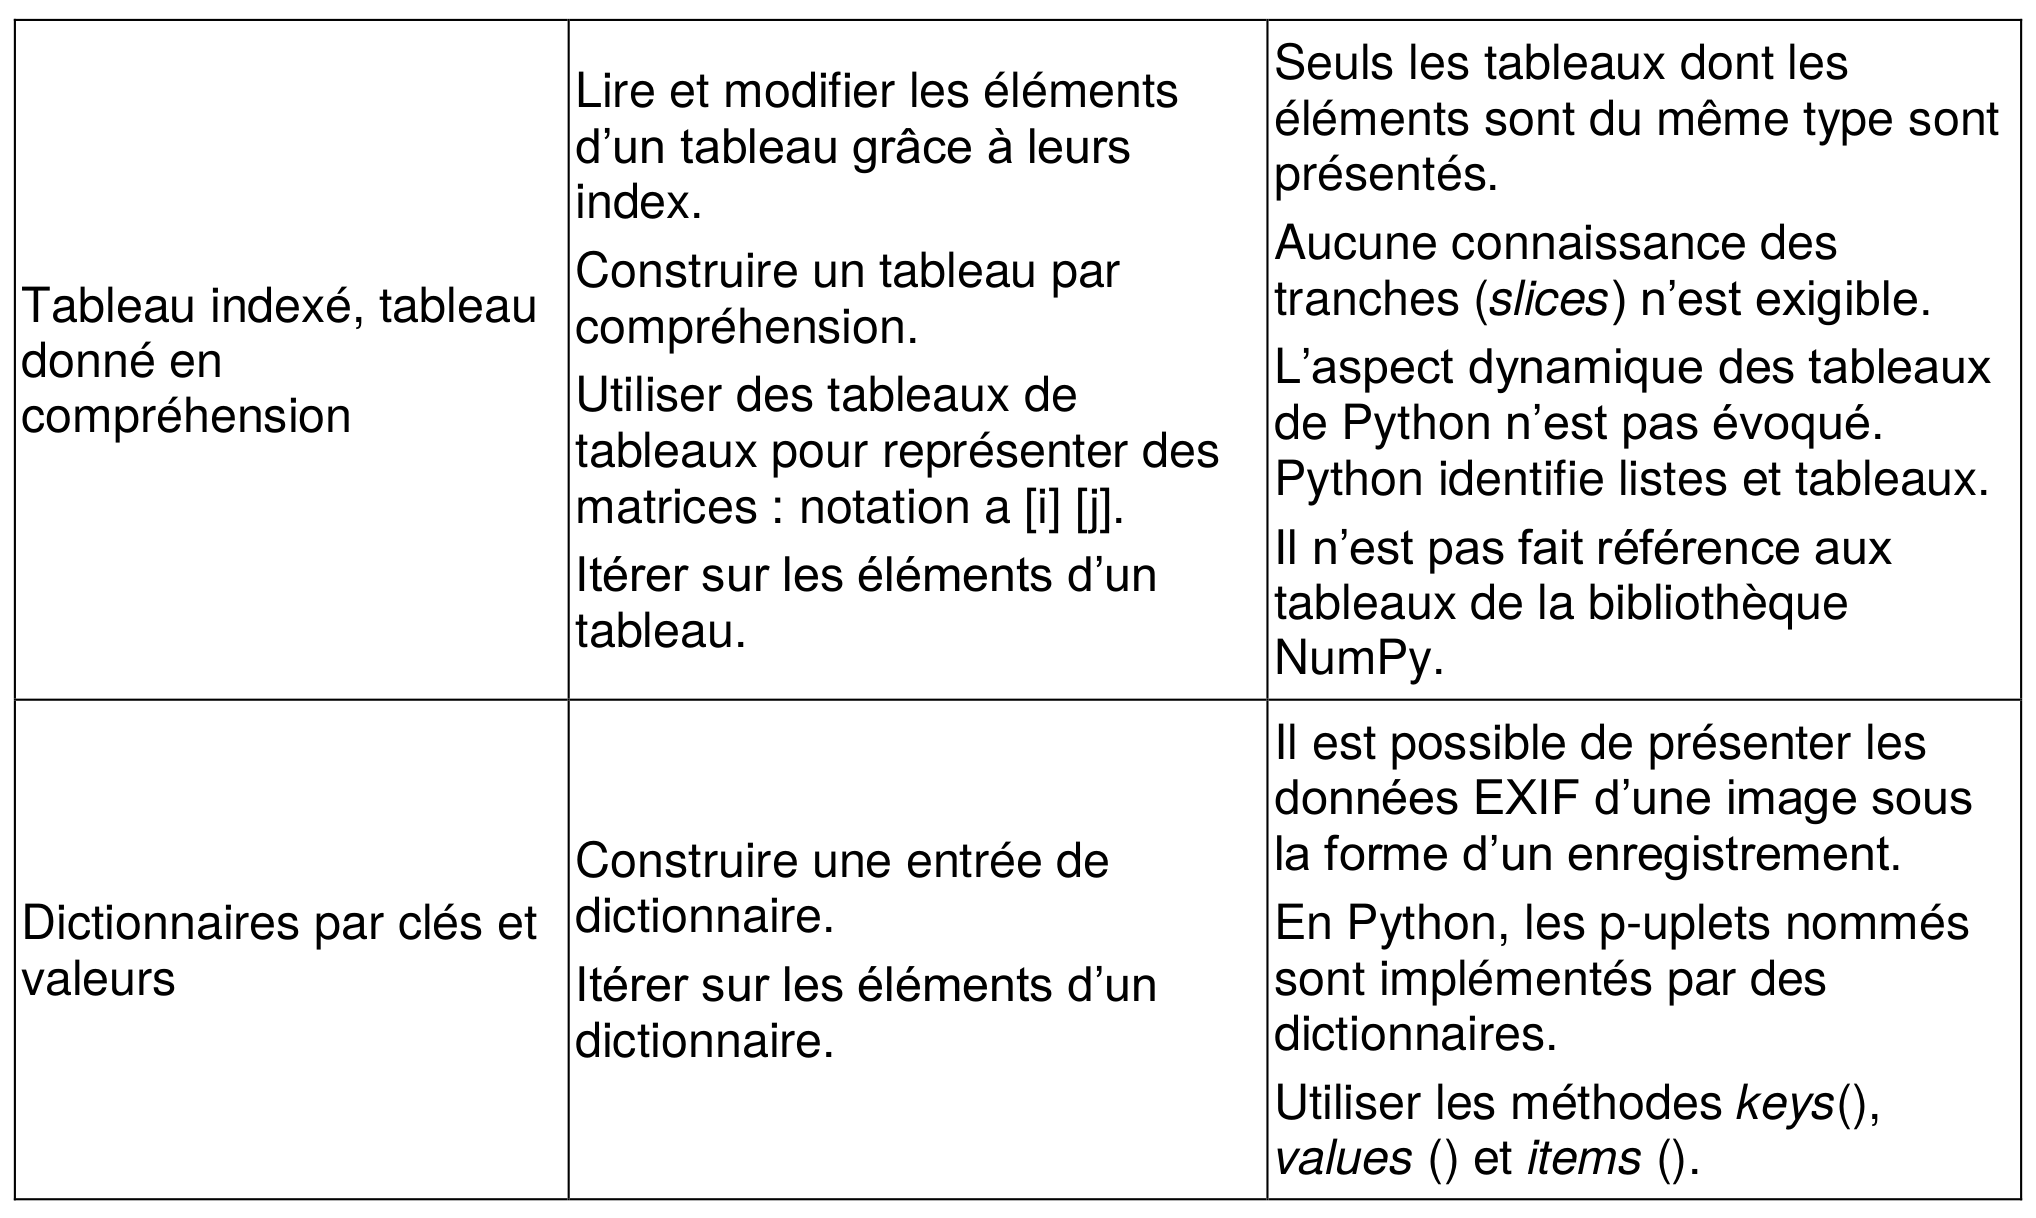
\includegraphics[width=10cm]{ressources/premiere.png}
    \end{center}

\end{frame}
\subsection{En terminale}
\begin{frame}
    \frametitle{En terminale}

    \begin{center}
        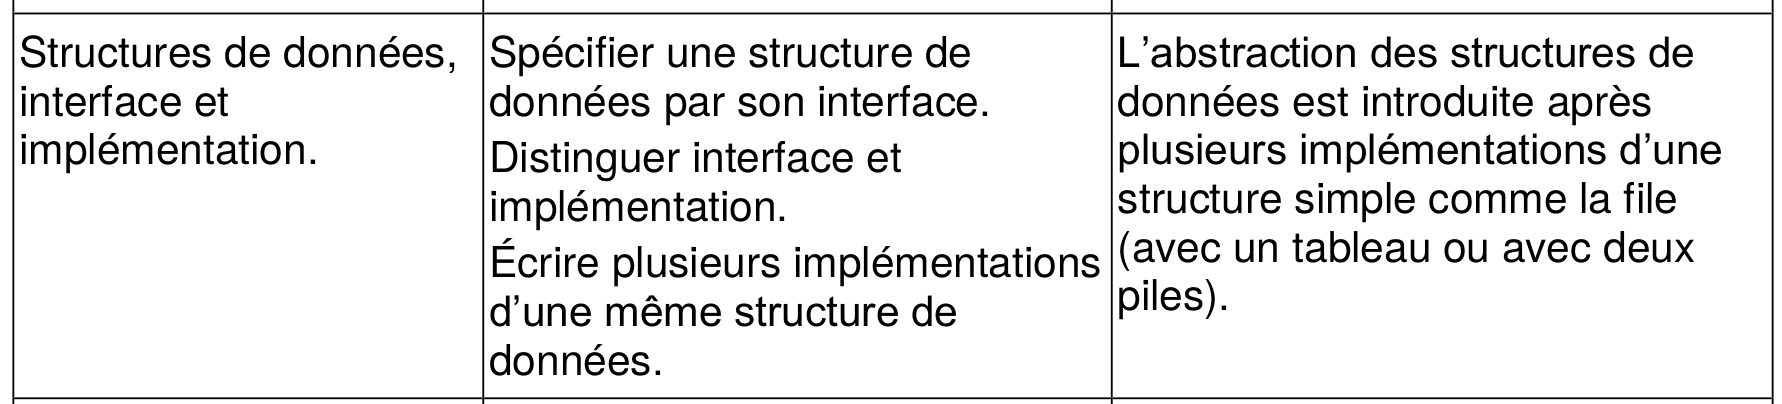
\includegraphics[width=10cm]{ressources/terminale1.png}
    \end{center}
    \begin{center}
        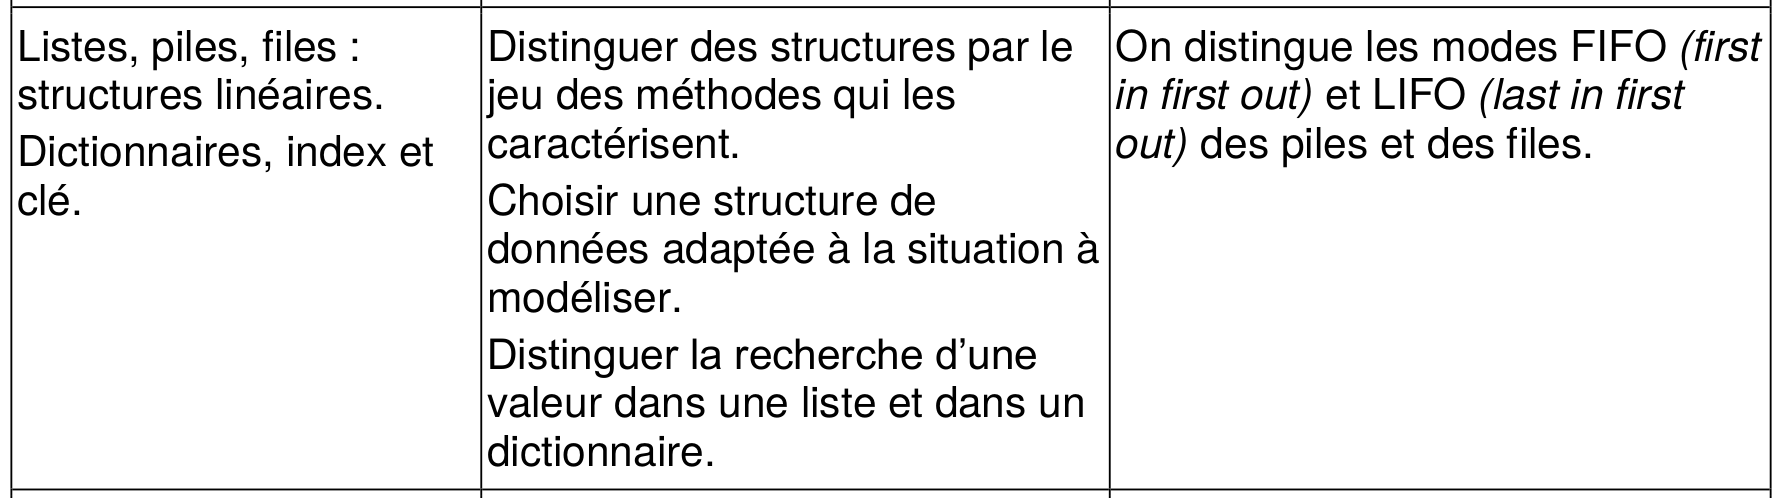
\includegraphics[width=10cm]{ressources/terminale2.png}
    \end{center}

\end{frame}
\section{Listes}
\subsection{Ambiguïté}
\begin{frame}
    \frametitle{Listes - Ambiguïté}


    \begin{aretenir}[Observation]
        \centering Les \textbf{\texttt{list}} Python ne sont pas des listes.
    \end{aretenir}
\end{frame}
\begin{frame}
    \frametitle{}

    \begin{aretenir}[Définition]
        \centering Une liste est une séquence ordonnée d'éléments de même type. Chaque élément est repéré par sa position dans la liste.
    \end{aretenir}

\end{frame}
\subsection{Tableau}
\subsubsection{Définition}
\begin{frame}
    \frametitle{Tableau - Définition}

    \begin{aretenir}[Définition]
        Un tableau est une séquence ordonnée et \underline{contigüe} d'éléments de même type.\\
        Le contenu d'un tableau est modifiable.
    \end{aretenir}

\end{frame}
\begin{frame}
    \frametitle{}

    \begin{center}
        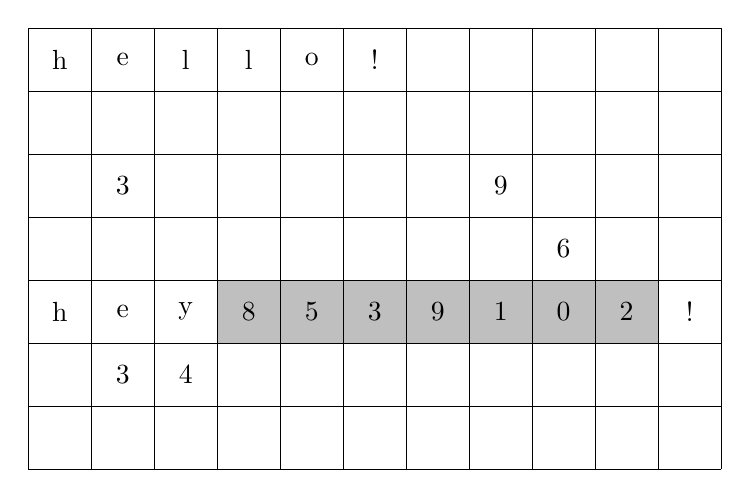
\begin{tikzpicture}[scale=0.8]
            \fill[gray!50] (3,2) rectangle (10,3);
            \draw (0,0) grid (11,7);

            \draw (0.5,2.5) node{h};
            \draw (1.5,2.5) node{e};
            \draw (2.5,2.5) node{y};

            \draw (0.5,6.5) node{h};
            \draw (1.5,6.5) node{e};
            \draw (2.5,6.5) node{l};
            \draw (3.5,6.5) node{l};
            \draw (4.5,6.5) node{o};
            \draw (5.5,6.5) node{!};

            \draw (10.5,2.5) node{!};
            \draw (7.5,4.5) node{9};
            \draw (8.5,3.5) node{6};
            \draw (1.5,4.5) node{3};
            \draw (2.5,1.5) node{4};
            \draw (1.5,1.5) node{3};

            \foreach \x/\y in {3/8,4/5,5/3,6/9,7/1,8/0,9/2}
                {\draw (\x+0.5,2.5) node{\y};}
        \end{tikzpicture}
        \captionof{figure}{\centering Simulation de représentation en mémoire}
        \label{IMG}
    \end{center}

\end{frame}
\subsubsection{Complexité temporelle}
\begin{frame}
    \frametitle{Complexité temporelle}

    \begin{center}
        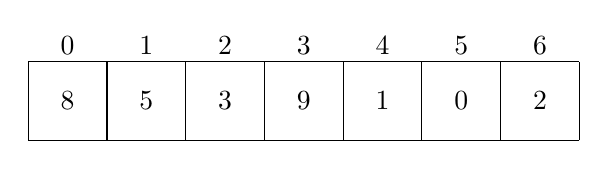
\begin{tikzpicture}
            \draw (0,0) grid (7,1);
            \foreach \x/\n in {0/8,1/5,2/3,3/9,4/1,5/0,6/2}{
                    \node at (0.5+\x, 1.2) {\x};
                    \node at (0.5+\x, .5) {\n};
                }
        \end{tikzpicture}
        \captionof{figure}{\centering On accède à un élément \textbf{en temps constant} grâce à son indice.}
    \end{center}


\end{frame}
\begin{frame}
    \frametitle{}
    \begin{center}
        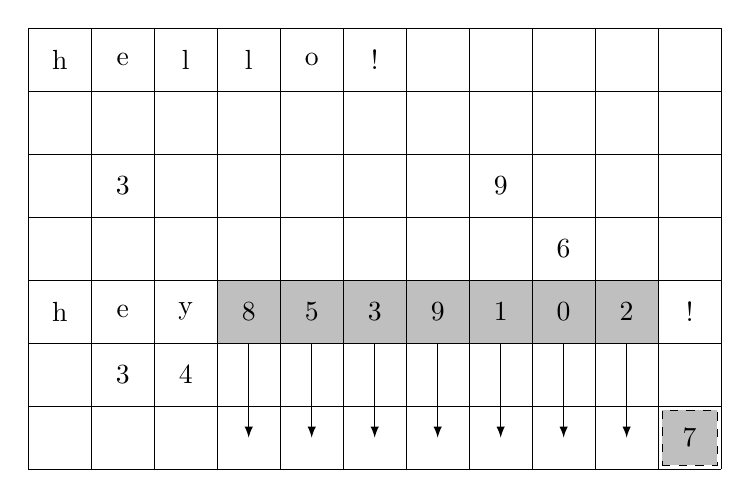
\begin{tikzpicture}[scale=0.8]
            \fill[gray!50] (3,2) rectangle (10,3);
            \draw (0,0) grid (11,7);

            \draw (0.5,2.5) node{h};
            \draw (1.5,2.5) node{e};
            \draw (2.5,2.5) node{y};

            \draw (0.5,6.5) node{h};
            \draw (1.5,6.5) node{e};
            \draw (2.5,6.5) node{l};
            \draw (3.5,6.5) node{l};
            \draw (4.5,6.5) node{o};
            \draw (5.5,6.5) node{!};

            \draw (10.5,2.5) node{!};
            \draw (7.5,4.5) node{9};
            \draw (8.5,3.5) node{6};
            \draw (1.5,4.5) node{3};
            \draw (2.5,1.5) node{4};
            \draw (1.5,1.5) node{3};

            \foreach \x/\y in {3/8,4/5,5/3,6/9,7/1,8/0,9/2}
                {\draw (\x+0.5,2.5) node{\y};
                    \draw[->,>=latex] (\x+.5,2) -- (\x+.5,.5);
                }
            \node[draw,dashed,fill=gray!50, minimum width=0.7cm,minimum height=0.7cm] at(10.5,.5) {7};
        \end{tikzpicture}
        \captionof{figure}{\centering Agrandir un tableau peut prendre \textbf{un temps linéaire} à la taille du tableau.}
        \label{IMG}
    \end{center}


\end{frame}
\subsection{Liste chaînée}
\subsubsection{Définition}
\begin{frame}
    \frametitle{Liste chaînée - Définition}

    \begin{aretenir}[Définition]
        Une liste chaînée est une séquence ordonnée où chaque élément possède une référence vers le suivant.
    \end{aretenir}

\end{frame}
\begin{frame}
    \frametitle{}

    \begin{center}
        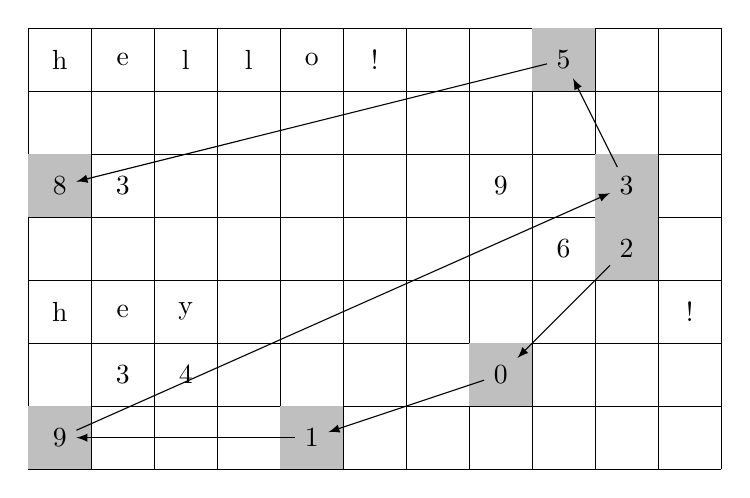
\begin{tikzpicture}[scale=0.8]
            \draw (0,0) grid (11,7);

            \draw (0.5,2.5) node{h};
            \draw (1.5,2.5) node{e};
            \draw (2.5,2.5) node{y};

            \draw (0.5,6.5) node{h};
            \draw (1.5,6.5) node{e};
            \draw (2.5,6.5) node{l};
            \draw (3.5,6.5) node{l};
            \draw (4.5,6.5) node{o};
            \draw (5.5,6.5) node{!};

            \draw (10.5,2.5) node{!};
            \draw (7.5,4.5) node{9};
            \draw (8.5,3.5) node{6};
            \draw (1.5,4.5) node{3};
            \draw (2.5,1.5) node{4};
            \draw (1.5,1.5) node{3};

            \fill[gray!50] (0,4) rectangle (1,5);
            \node (8) at (0.5,4.5) {8};
            \fill[gray!50] (8,6) rectangle (9,7);
            \node (5) at (8.5,6.5) {5};
            \fill[gray!50] (9,4) rectangle (10,5);
            \node (3) at (9.5,4.5) {3};
            \fill[gray!50] (0,0) rectangle (1,1);
            \node (9) at (0.5,0.5) {9};
            \fill[gray!50] (4,0) rectangle (5,1);
            \node (1) at (4.5,0.5) {1};
            \fill[gray!50] (7,1) rectangle (8,2);
            \node (0) at (7.5,1.5) {0};
            \fill[gray!50] (9,3) rectangle (10,4);
            \node (2) at (9.5,3.5) {2};
            \draw[<-,>=latex] (8) -- (5);
            \draw[<-,>=latex] (5) -- (3);
            \draw[<-,>=latex] (3) -- (9);
            \draw[<-,>=latex] (9) -- (1);
            \draw[<-,>=latex] (1) -- (0);
            \draw[<-,>=latex] (0) -- (2);
        \end{tikzpicture}
        \captionof{figure}{\centering Simulation de représentation en mémoire}
    \end{center}

\end{frame}
\subsubsection{Complexité temporelle}
\begin{frame}
    \frametitle{Complexité temporelle}

    \begin{center}
        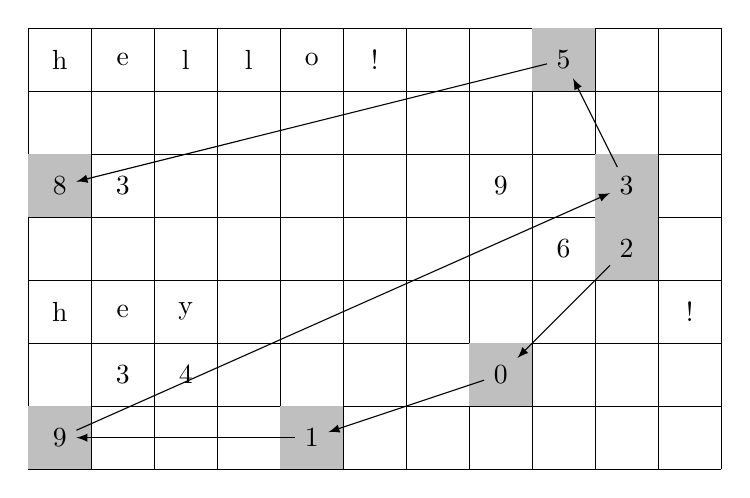
\begin{tikzpicture}[scale=0.8]
            \draw (0,0) grid (11,7);

            \draw (0.5,2.5) node{h};
            \draw (1.5,2.5) node{e};
            \draw (2.5,2.5) node{y};

            \draw (0.5,6.5) node{h};
            \draw (1.5,6.5) node{e};
            \draw (2.5,6.5) node{l};
            \draw (3.5,6.5) node{l};
            \draw (4.5,6.5) node{o};
            \draw (5.5,6.5) node{!};

            \draw (10.5,2.5) node{!};
            \draw (7.5,4.5) node{9};
            \draw (8.5,3.5) node{6};
            \draw (1.5,4.5) node{3};
            \draw (2.5,1.5) node{4};
            \draw (1.5,1.5) node{3};

            \fill[gray!50] (0,4) rectangle (1,5);
            \node (8) at (0.5,4.5) {8};
            \fill[gray!50] (8,6) rectangle (9,7);
            \node (5) at (8.5,6.5) {5};
            \fill[gray!50] (9,4) rectangle (10,5);
            \node (3) at (9.5,4.5) {3};
            \fill[gray!50] (0,0) rectangle (1,1);
            \node (9) at (0.5,0.5) {9};
            \fill[gray!50] (4,0) rectangle (5,1);
            \node (1) at (4.5,0.5) {1};
            \fill[gray!50] (7,1) rectangle (8,2);
            \node (0) at (7.5,1.5) {0};
            \fill[gray!50] (9,3) rectangle (10,4);
            \node (2) at (9.5,3.5) {2};
            \draw[<-,>=latex] (8) -- (5);
            \draw[<-,>=latex] (5) -- (3);
            \draw[<-,>=latex] (3) -- (9);
            \draw[<-,>=latex] (9) -- (1);
            \draw[<-,>=latex] (1) -- (0);
            \draw[<-,>=latex] (0) -- (2);
        \end{tikzpicture}
        \captionof{figure}{\centering On accède à l'élément de rang \textbf{\texttt{n}} \textbf{en temps linéaire}.}
    \end{center}
\end{frame}

\begin{frame}
    \frametitle{}

    \begin{center}
        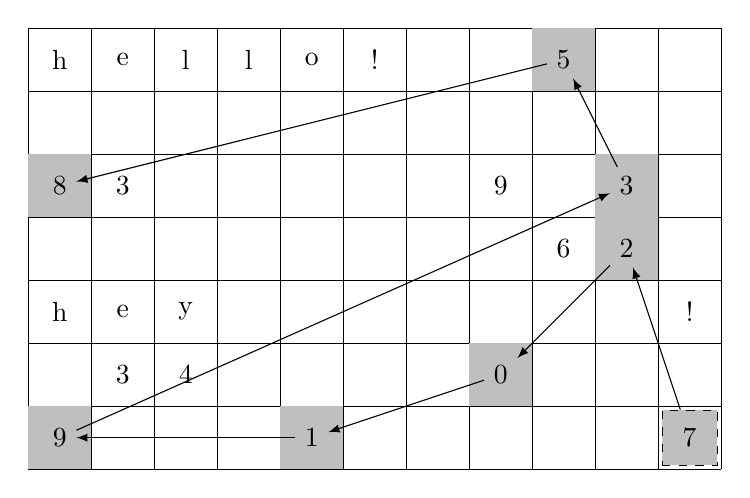
\begin{tikzpicture}[scale=0.8]
            \draw (0,0) grid (11,7);

            \draw (0.5,2.5) node{h};
            \draw (1.5,2.5) node{e};
            \draw (2.5,2.5) node{y};

            \draw (0.5,6.5) node{h};
            \draw (1.5,6.5) node{e};
            \draw (2.5,6.5) node{l};
            \draw (3.5,6.5) node{l};
            \draw (4.5,6.5) node{o};
            \draw (5.5,6.5) node{!};

            \draw (10.5,2.5) node{!};
            \draw (7.5,4.5) node{9};
            \draw (8.5,3.5) node{6};
            \draw (1.5,4.5) node{3};
            \draw (2.5,1.5) node{4};
            \draw (1.5,1.5) node{3};

            \fill[gray!50] (0,4) rectangle (1,5);
            \node (8) at (0.5,4.5) {8};
            \fill[gray!50] (8,6) rectangle (9,7);
            \node (5) at (8.5,6.5) {5};
            \fill[gray!50] (9,4) rectangle (10,5);
            \node (3) at (9.5,4.5) {3};
            \fill[gray!50] (0,0) rectangle (1,1);
            \node (9) at (0.5,0.5) {9};
            \fill[gray!50] (4,0) rectangle (5,1);
            \node (1) at (4.5,0.5) {1};
            \fill[gray!50] (7,1) rectangle (8,2);
            \node (0) at (7.5,1.5) {0};
            \fill[gray!50] (9,3) rectangle (10,4);
            \node (2) at (9.5,3.5) {2};
            \draw[<-,>=latex] (8) -- (5);
            \draw[<-,>=latex] (5) -- (3);
            \draw[<-,>=latex] (3) -- (9);
            \draw[<-,>=latex] (9) -- (1);
            \draw[<-,>=latex] (1) -- (0);
            \draw[<-,>=latex] (0) -- (2);

            \node[draw,dashed,fill=gray!50, minimum width=0.7cm,minimum height=0.7cm] (7) at(10.5,.5) {7};
            \draw[<-,>=latex] (2) -- (7);
        \end{tikzpicture}
        \captionof{figure}{\centering On ajoute un élément en tête de liste \textbf{en temps constant}.}
    \end{center}
\end{frame}
\subsection{\textbf{\texttt{list} Python}}
\begin{frame}
    \frametitle{\textbf{\texttt{list} Python}}

    \begin{aretenir}[Observations]
        \begin{itemize}
            \item Python est un langage de haut-niveau.
            \item Les \textbf{\texttt{list}} essaie de prendre les avantages des deux structures précédentes.
            \item Les \textbf{\texttt{list}} vont plus loin: les éléments peuvent être de types différents.
        \end{itemize}
    \end{aretenir}

\end{frame}
\section{Parcours de listes et dictionnaires}
\subsection{Difficultés rencontrées}
\begin{frame}
    \frametitle{Parcours de listes et dictionnaires - Difficultés rencontrées}

    \begin{aretenir}[Constat]
\begin{itemize}
    \item Dans un tableau, confusion indice / élément.
    \item Tentative de récupération des informations dans un dictionnaire, avec un indice.
\end{itemize}
    \end{aretenir}
\end{frame}
\begin{frame}[fragile]
    \frametitle{}

\begin{center}
\begin{lstlisting}[language=Python , basicstyle=\ttfamily\small, xleftmargin=2em, xrightmargin=2em]
# confusion indice / élément
tab = [3, 9, 1]
for i in tab:
    print(tab[i])
\end{lstlisting}
\begin{lstlisting}[language=Python , basicstyle=\ttfamily\small, xleftmargin=2em, xrightmargin=2em]
# indice dans un dictionnaire
dico = {"a": 2, "e": 4, "f": 1}
for i in range(len(dico)):
    print(dico[i])
\end{lstlisting}
\captionof{code}{Erreurs courantes}
\label{CODE}
        \end{center}
\end{frame}
\subsection{Surmonter les difficultés}
\begin{frame}
    \frametitle{Surmonter les difficultés}

    \begin{center}
        \begin{tikzpicture}[scale=0.8]
            \draw (0,0) grid (5,1);

            \draw (0.5,2.5) node{h};
            \draw (1.5,2.5) node{e};
            \draw (2.5,2.5) node{y};

            \draw (0.5,6.5) node{h};
            \draw (1.5,6.5) node{e};
            \draw (2.5,6.5) node{l};
            \draw (3.5,6.5) node{l};
            \draw (4.5,6.5) node{o};
            \draw (5.5,6.5) node{!};

            \draw (10.5,2.5) node{!};
            \draw (7.5,4.5) node{9};
            \draw (8.5,3.5) node{6};
            \draw (1.5,4.5) node{3};
            \draw (2.5,1.5) node{4};
            \draw (1.5,1.5) node{3};
        \end{tikzpicture}
        \captionof{figure}{\centering On accède à l'élément de rang \textbf{\texttt{n}} \textbf{en temps linéaire}.}
    \end{center}

\end{frame}

\section{Fonction et paramètre mutable}
\begin{frame}
    \frametitle{Fonction et paramètre mutable}
valeur par défaut dans paramètre
    

\end{frame}
\section{Piles, files}
\subsection{Définition}
\subsection{Interface}
\subsection{Implémentations}
\subsubsection{Par un tableau}
\subsubsection{Par une liste chaînée}
\end{document}